\section{Конструкторский раздел \hfill}
\vspace{\baselineskip}

\subsection{Разработка конвейера}

Алгоритм раскраски графа по количеству смежных вершин можно разделить на 3 этапа:
\begin{enumerate}
    \item вычисление числа соседей каждого узла;
    \item составление описания графа для graphviz;
    \item вывод описания графа в файл с расширением dot.
\end{enumerate}

Таким образом, конвейер состоит из 3 лент, каждая из которых выполняет соответствующий этап. 

\subsection{Разработка алгоритмов}

На рисунках \ref{fig:count_neighbors}-\ref{fig:write_to_file} представлены схемы этапов алгоритма раскраски графа по количеству смежных вершин. 

На рисунке \ref{fig:linear} приведена схема линейного алгоритма раскраски графа по количеству смежных вершин.

На рисунках \ref{fig:parallel}-\ref{fig:parallel_3} представлены схемы алгоритма раскраски графа с использованием конвейерных вычислений.

\clearpage

\begin{figure}[h!btp]
	\centering
	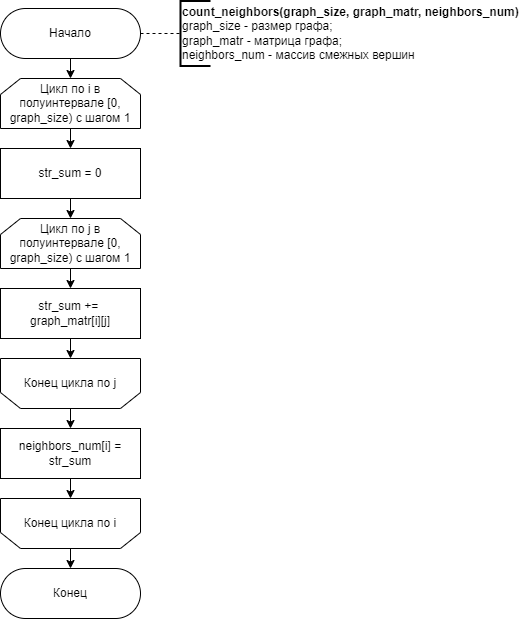
\includegraphics[width=360pt]{inc/count_neighbors.png}
	\caption{Схема этапа вычисления числа соседей каждого узла}
	\label{fig:count_neighbors}	
\end{figure}

\clearpage

\begin{figure}[h!btp]
	\centering
	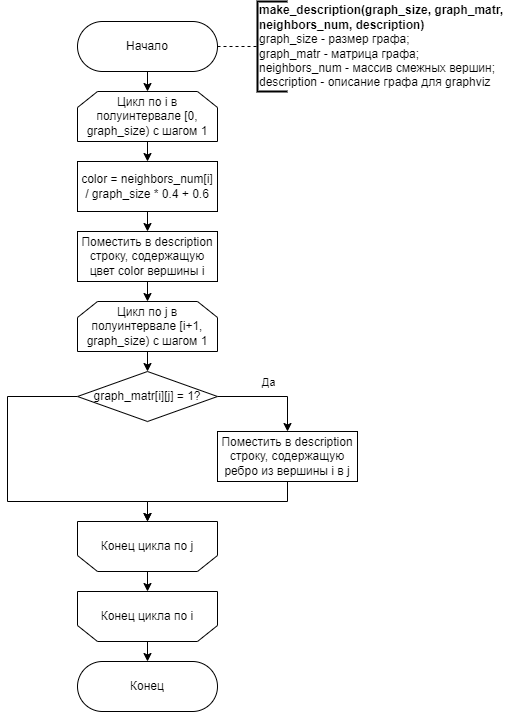
\includegraphics[width=360pt]{inc/make_description.png}
	\caption{Схема этапа составления описания графа для graphviz}
	\label{fig:make_description}	
\end{figure}

\clearpage

\begin{figure}[h!btp]
	\centering
	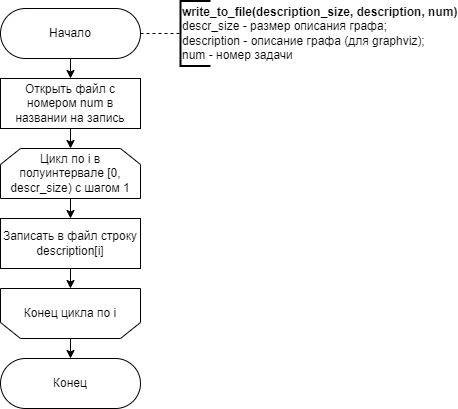
\includegraphics[width=360pt]{inc/write_to_file.png}
	\caption{Схема этапа вывода описания графа в файл с расширением dot}
	\label{fig:write_to_file}	
\end{figure}

\clearpage

\begin{figure}[h!btp]
	\centering
	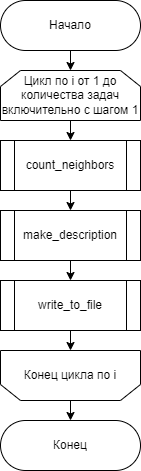
\includegraphics[width=120pt]{inc/linear.png}
	\caption{Схема линейного алгоритма раскраски графов}
	\label{fig:linear}	
\end{figure}

\clearpage

\begin{figure}[h!btp]
	\centering
	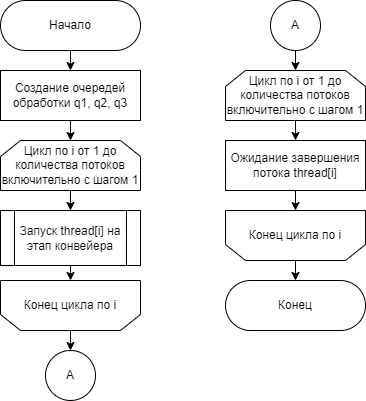
\includegraphics[width=240pt]{inc/parallel.png}
	\caption{Схема работы главного потока для реализации алгоритма раскраски графа с использованием конвейера}
	\label{fig:parallel}	
\end{figure}

\begin{figure}[h!btp]
	\centering
	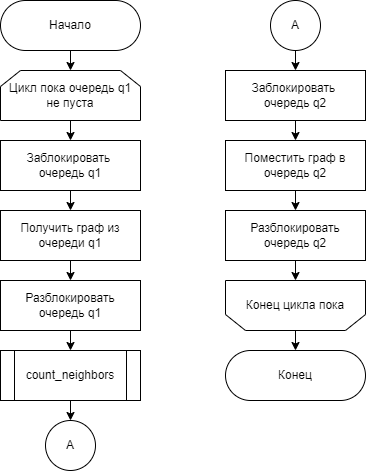
\includegraphics[width=240pt]{inc/parallel_1.png}
	\caption{Схема работы потока на первом этапе конвейерных вычислений}
	\label{fig:parallel_1}	
\end{figure}

\clearpage

\begin{figure}[h!btp]
	\centering
	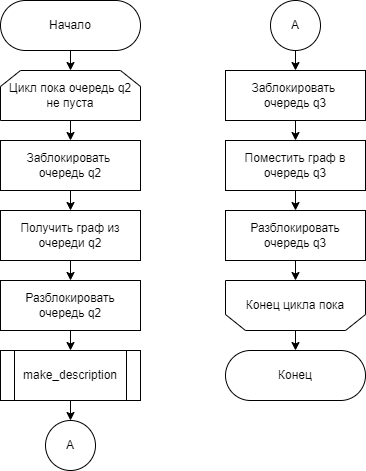
\includegraphics[width=240pt]{inc/parallel_2.png}
	\caption{Схема работы потока на втором этапе конвейерных вычислений}
	\label{fig:parallel_2}	
\end{figure}

\begin{figure}[h!btp]
	\centering
	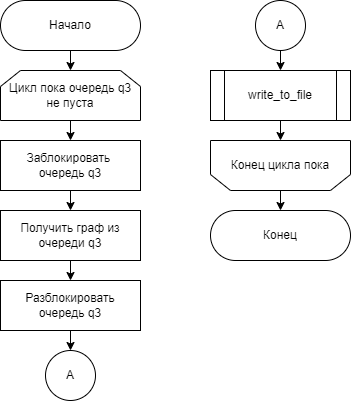
\includegraphics[width=240pt]{inc/parallel_3.png}
	\caption{Схема работы потока на третьем этапе конвейерных вычислений}
	\label{fig:parallel_3}	
\end{figure}

\clearpage

\subsection*{Вывод}

Были описаны структура и принцип работы разрабатываемого конвейра, а также приведены схемы разрабатываемых алгоритмов.
